\documentclass[pdflatex,compress,mathserif]{beamer}

%\usetheme[dark,framenumber,totalframenumber]{ElektroITK}
\usetheme[darktitle,framenumber,totalframenumber]{ElektroITK}

\usepackage[utf8]{inputenc}
\usepackage[T1]{fontenc}
\usepackage{lmodern}
\usepackage[bahasai]{babel}
\usepackage{amsmath}
\usepackage{amsfonts}
\usepackage{amssymb}
\usepackage{graphicx}
\usepackage{multicol}

\newcommand*{\Scale}[2][4]{\scalebox{#1}{$#2$}}%

\title{PEMODELAN JARINGAN KOMUNIKASI}
\subtitle{VLANs - Virtual Local Area Networks}

\author{Tim Dosen Pengampu}

\begin{document}
	
\maketitle

\section{Campus Design - Access, Distribution and Core Layers}

\begin{frame}
	\frametitle{Campus Design - Access, Distribution and Core Layers}
	\begin{itemize}
		\item The campus LAN should be designed for scalability, performance and
security
		\item To aid in a best practice design process, the network topology is split
into access, distribution and core layers
		\item The layers have their own design principles and characteristics
	\end{itemize}
\end{frame}

\begin{frame}
	\frametitle{Campus Design – Access Layer}
	\begin{center}
		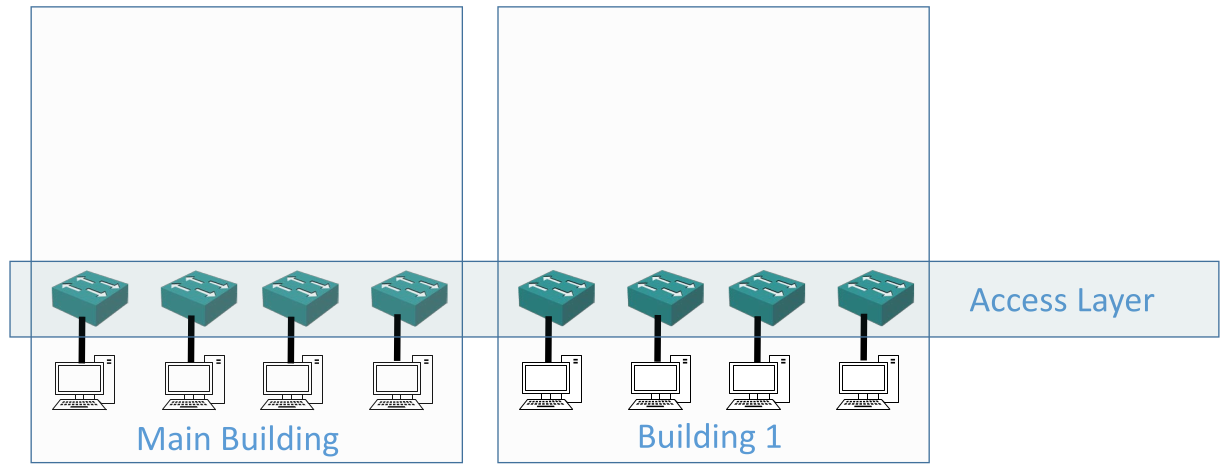
\includegraphics[width=\linewidth]{img/img01}
	\end{center}
\end{frame}

\begin{frame}
	\frametitle{The Access Layer}
	\begin{itemize}
		\item End hosts such as desktop computers, servers and IP phones connect
into the network at the access layer
		\item It is designed to have a high port count at an affordable cost
		\item Desktops typically have only one Network Interface Card (NIC) so they
connect into one switch or Wireless Access Point
		\item Servers will often have dual NICs and connect to a pair of redundant
switches
		\item Client access security measures are enabled at the Access Layer
	\end{itemize}
\end{frame}

\begin{frame}
	\frametitle{Campus Design - Distribution Layer}
	\begin{center}
		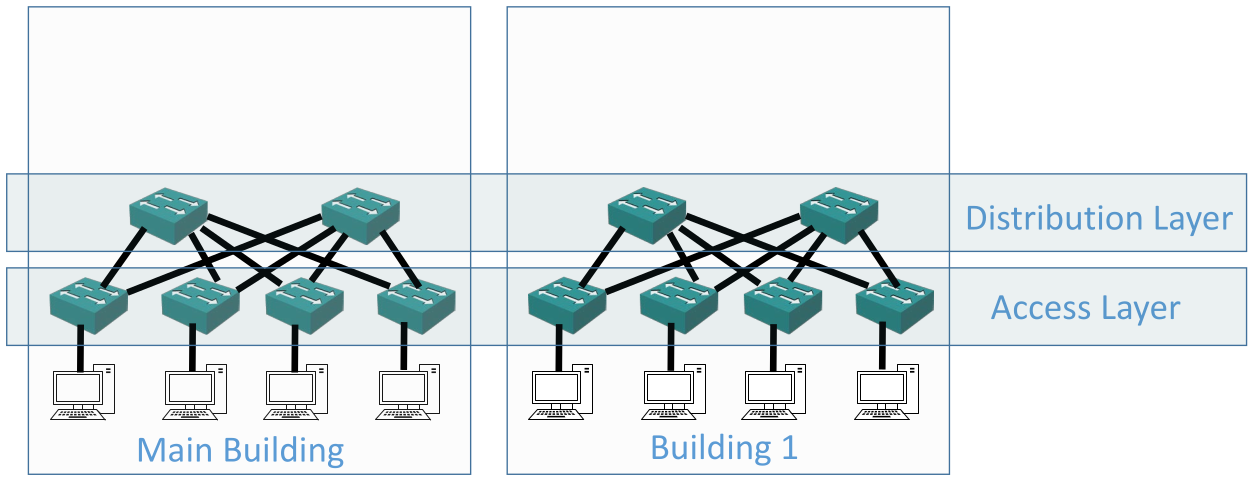
\includegraphics[width=\linewidth]{img/img02}
	\end{center}
\end{frame}

\begin{frame}
	\frametitle{The Distribution Layer}
	\begin{itemize}
		\item Access Layer switches uplink to Distribution Layer switches
		\item The Distribution Layer switches serve as an aggregation point for the
Access Layer and provide scalability
		\item Distribution Layer switches are typically deployed in redundant pairs,
with downstream Access Layer switches connected to both
		\item End hosts are not typically connected here
		\item Most software policy such as QoS is enabled at this layer
	\end{itemize}
\end{frame}

\begin{frame}
	\frametitle{Campus Design - Core Layer}
	\begin{center}
		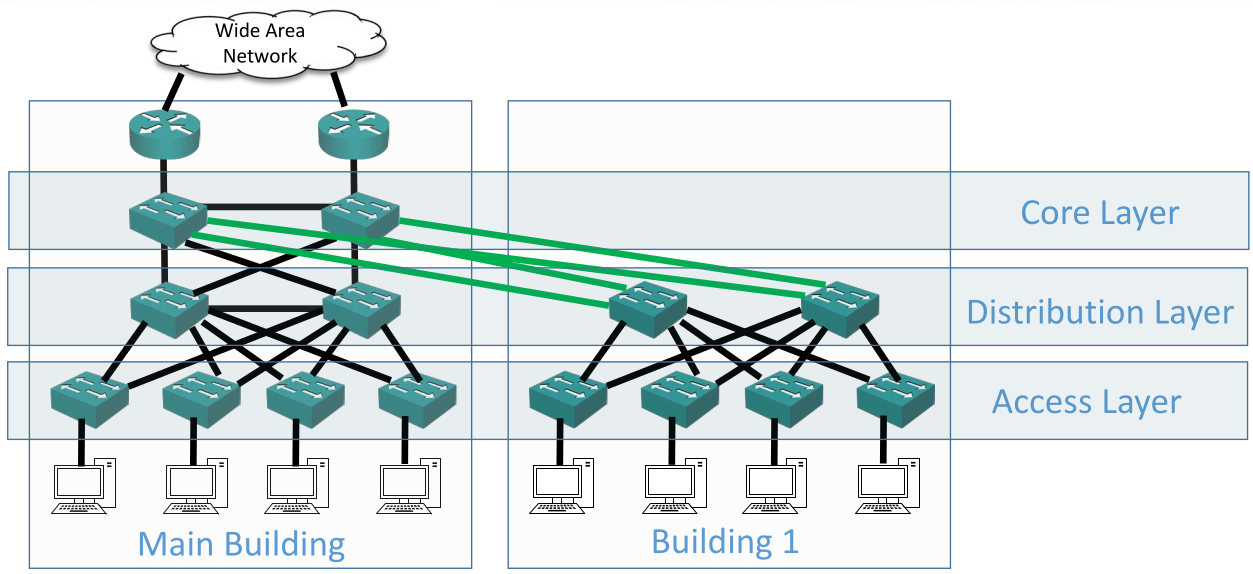
\includegraphics[width=\linewidth]{img/img03}
	\end{center}
\end{frame}

\begin{frame}
	\frametitle{The Core Layer}
	\begin{itemize}
		\item Distribution Layer switches uplink to Core Layer switches
		\item Core Layer switches are typically deployed in redundant pairs, with
downstream Distribution Layer switches connected to both
		\item Traffic between different parts of the campus travels through the core
so it is designed for speed and resiliency
		\item Software policy slows the switch down so should be avoided in the
Core Layer
	\end{itemize}
\end{frame}

\begin{frame}
	\frametitle{Collapsed Distribution and Core}
	\begin{itemize}
		\item Smaller campuses do not need the scalability of three separate layers
		\item In these cases a Collapsed Distribution and Core layer is used, where
the Distribution and Core layer functions are performed on the same
hardware device
	\end{itemize}
\end{frame}

\begin{frame}{Collapsed Distribution and Core}
	\begin{center}
		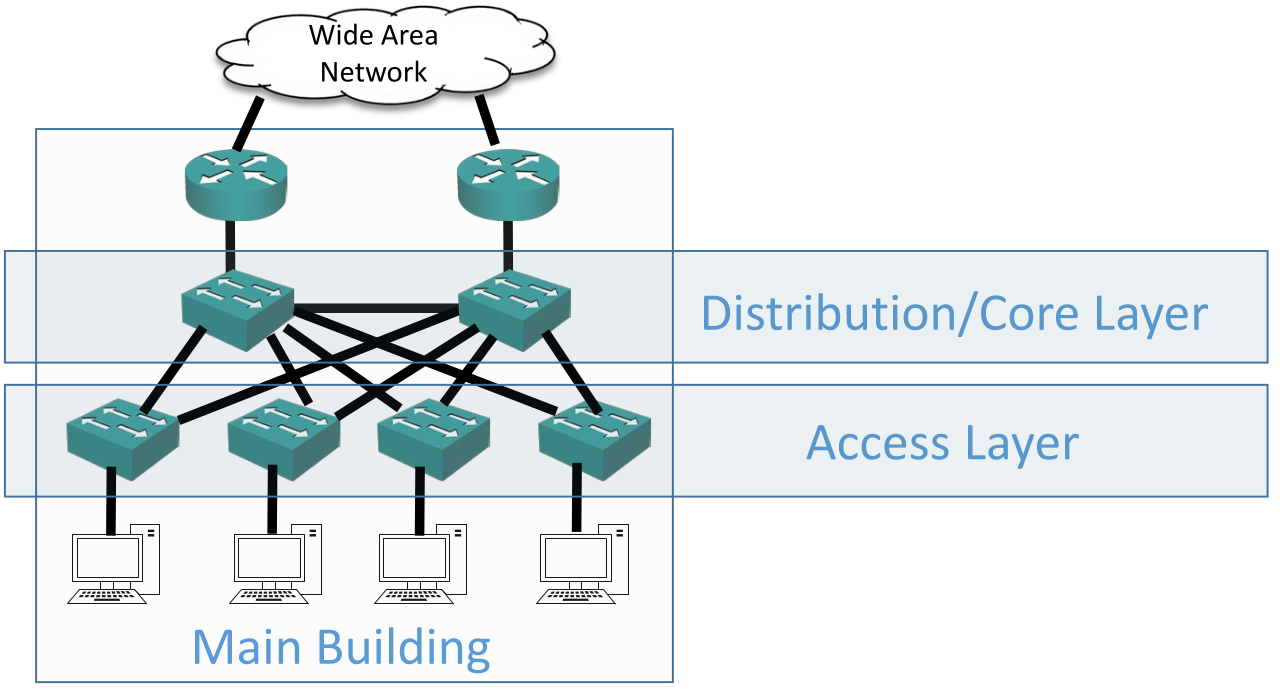
\includegraphics[width=\linewidth]{img/img04}
	\end{center}
\end{frame}

\section{Spine-Leaf Network Design}

\section{Why we have VLANs}

\section{VLAN Access Ports}

\section{VLAN Trunk Ports}

\section{DTP Dynamic Trunking Protocol}

\section{VTP VLAN Trunking Protocol}

\end{document}